\section{Governing equations}\label{sec:governing_equations}

In this section the governing equations of the problem described in \sref{sec:problem_definition} are detailed.

\subsection{Hypothesis}

\begin{itemize}
\item All orbits are contained in the same plane.
\item Earth and Jupiter orbits are circular with radius $r_c$ defined as \eref{eq:radi_mig}.

\begin{equation}\label{eq:radi_mig}
d_c = \frac{d_a + d_p}{2}
\end{equation}

\item $\Delta V$ to escape from Earth is applied at a certain time which achieves that the initial velocity of the vehicle's orbit around the Sun is tangent to the Earth's orbit around the Sun.

\item Neglect the initial altitude when approaching and leaving a planet. Radius of sphere of influence $r_{SOI}$: $$r_{SOI} = 0 \si{[km]}$$
\end{itemize}

\subsection{Scape maneuver} \label{sec:scape_maneuver}

To begin the study an initial $\Delta V_{i}$ needed to scape the orbit of Earth and enter into an elliptical orbit around the Sun will be considered.

%%\subsubsection{Earth to Jupiter with two thrusts}\label{sec:two_thrusts}
\begin{figure}[H]
	\centering
		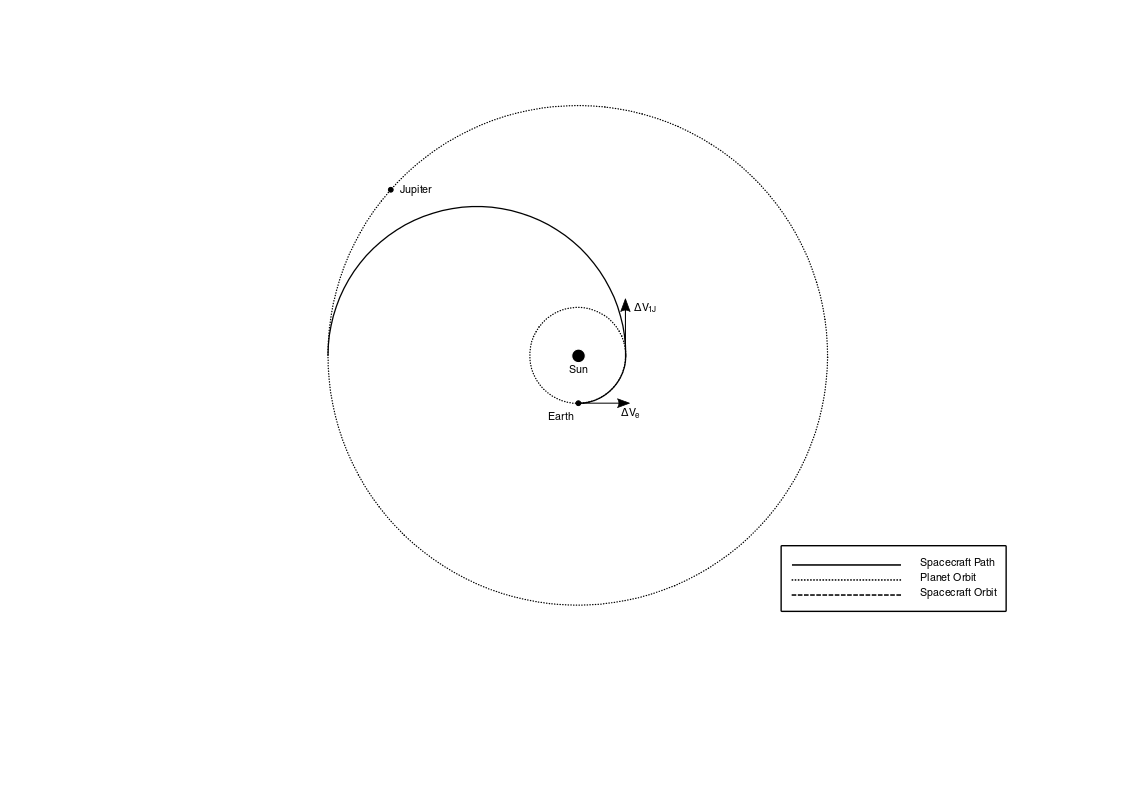
\includegraphics[width=\textwidth]{parabolica.png}
	\caption{Earth to Jupiter with two $\Delta V$}
	\label{fig:parabolica}
\end{figure}

The objective is to reach an elliptical orbit around the Sun whose apoapsis radius equals Jupiter's orbital radius. The starting point is  a satellite orbiting Earth at a determined $H_0$. In order to achieve this, two thrusts will be applied. 

\begin{itemize}
\item The first thrust will make the vehicle escape Earth's sphere of influence with a parabolic orbit. This can be calculated by substracting the speed of the satellite ($V_{s}$) from the Earth's scape velocity ($V_{e}$). To calculate $\Delta V_{e}$ it is imposed that the mechanical energy with respect to Earth equals zero at infinity.

\begin{equation}\label{eq:thrust}
\Delta V_e = V_e - V_s = \sqrt{\frac{2\mu_E}{R_E + H_0}}-\sqrt{\frac{\mu_E}{R_E+H_0}}
\end {equation}

After this first thrust, relative speed between Earth and the spacecraft will be zero, hence spacecraft's speed relative to the Sun will be the same as Earth's. Therefore, once this thrust has been applied, the vehicle will describe a circular orbit around the Sun whose radius will be equal to Earth's orbital radius. This thrust depends on initial $H_0$, as shown in . %%ref to figure 1 

\item A second thrust is used to bring the spacecraft to an elliptical orbit from a circular one. The desired orbital apoapsis radius equals Jupiter's orbital radius. It is important to realize that this latter thrust doesn't depend on $H_0$. In order to calculate this, the speed of the satellite in the circular orbit is substracted from the speed at periapsis of the ellipse.



\begin{equation}\label{eq:DV1J}
\Delta V_{1J} = V_{elliptical}-V_{circular} = \sqrt {\mu_{Sun}\left(\frac{2}{d_{SE}}-\frac{1}{a}\right)}-\sqrt{\frac{\mu_{Sun}}{d_{SE}}}
\end{equation}

Where $a = \frac{d_{SE} + d_{SJ}}{2}$

\end{itemize}

\fref{fig:parabolica} shows approximately the maneuver, although the initial orbit around Earth cannot be appreciated.\\

Total needed thrust to perform this maneuver will be the result of adding the two previously calculated thrusts.

\begin{equation*}\label{eq:impuls1T}
\Delta V_{1T} = \Delta V_e + \Delta V_{1J}
\end{equation*}

\begin{figure}[H]
	\centering
		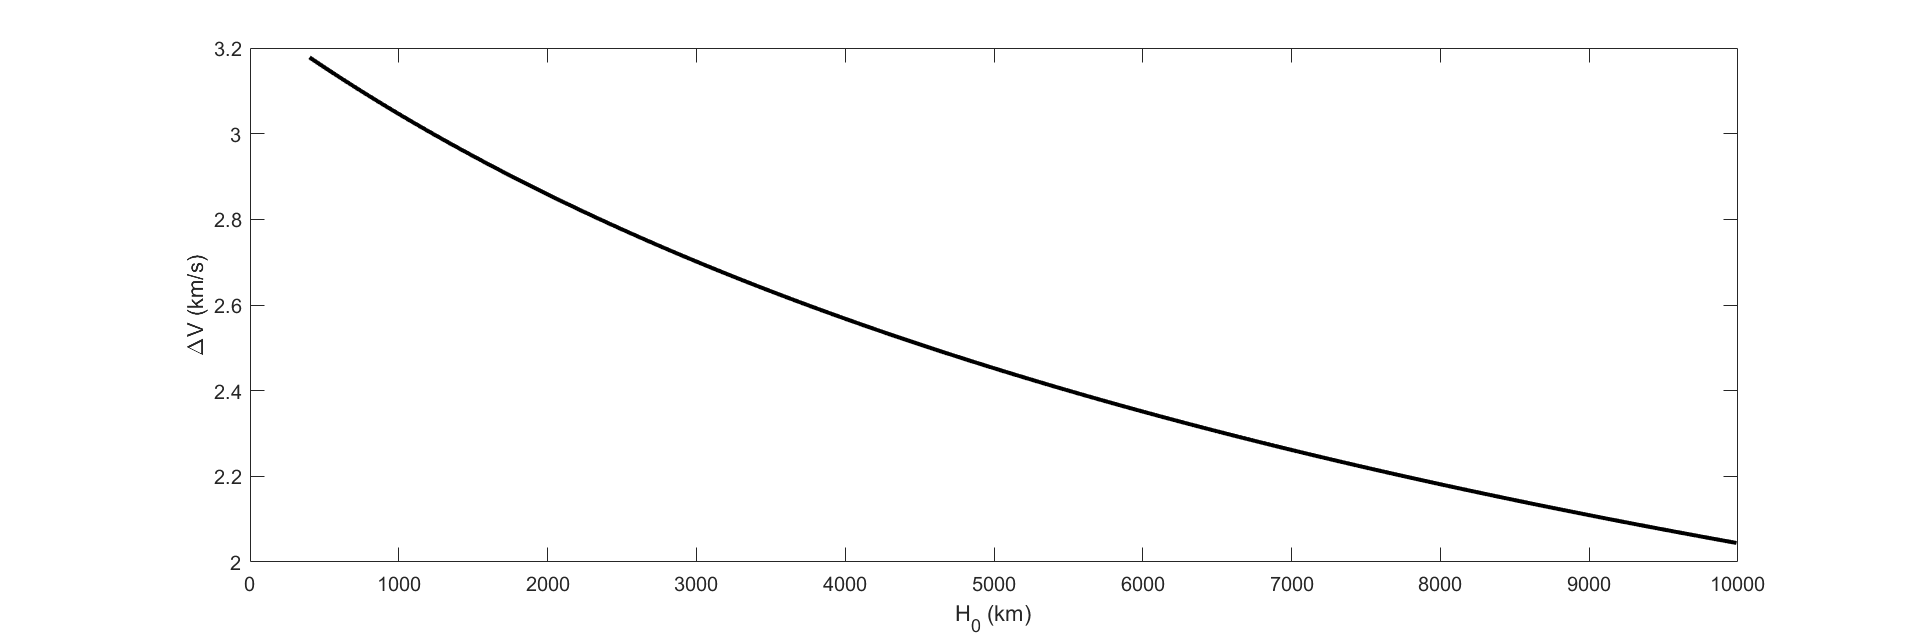
\includegraphics[width=\textwidth]{1a.png}
	\caption{$\Delta V$ vs $H_0$}
	\label{fig:1a}
\end{figure}


\subsection{Elliptic orbit}

\begin{figure}[H]
	\centering
		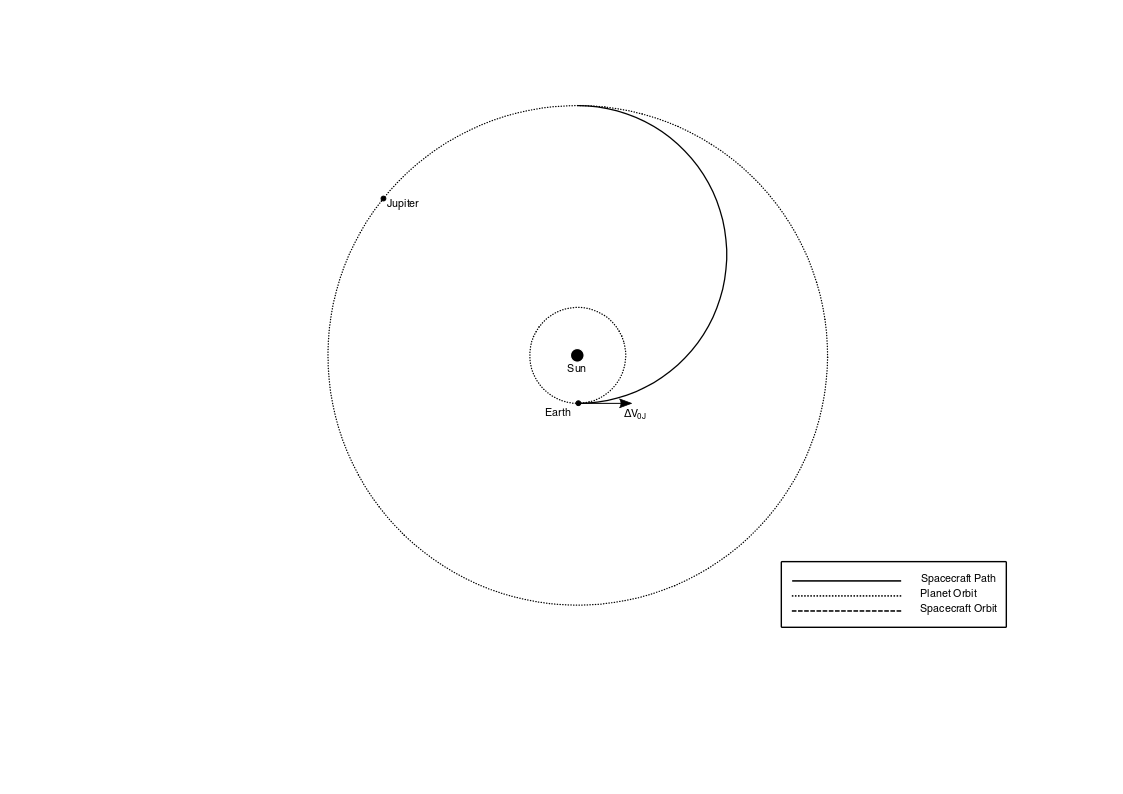
\includegraphics[width=\textwidth]{directa.png}
	\caption{Earth to Jupiter with one $\Delta V$}
	\label{fig:direct}
\end{figure}


The objective here is, again, escaping the Earth and orbit the Sun with an apoapsis radius equal to Jupiter's orbital radius ($r_a = d_{SJ}$). This time, however, just one thrust will be applied.

To do so, the spacecraft has to escape the Earth following a hyperbolic path, and enter, in consequence, an elliptical orbit around the Sun. The periapsis of this orbit will be at the point where the thrust is given, as shown in~\fref{fig:direct}

According to the conservation of energy, mechanical energy must remain constant. Therefore, the energy at the periapsis (where thrust maneuver is performed) is the same as the kinetic energy caused by the speed excess with respect to Earth ($V_\infty$). Thus, equation~\ref{eq:energy} is found by adding potential and kinetic in orbit energy of the spacecraft and equaling that to kinetic energy at infinity.

\begin{equation}\label{eq:energy}
E=\frac{\mu_{E}}{R_E + H_0} + \frac{(V_s + \Delta V_{0J})^2}{2}=\frac{(V_{\infty})^2}{2}
\end{equation}

As obtained $V_\infty$ is refered to Earth, the  orbital speed of the vehicle around the Sun will be calculated ($V_e$) by adding $V_\infty$ to Earth's orbital speed.
$\Delta V_{0J}$ is found by making $V_e$ equal to the vehicle's speed at an orbit around the Sun with $r_a = d_{SJ}$.

\begin{equation}\label{eq:thrust22}
\Delta V=\sqrt{\left(\sqrt{\mu_{Sun}\left(\frac{2}{d_{SE}}-\frac{1}{a}\right)}-\sqrt{\frac{\mu_{Sun}}{d_{SE}}}\right)^2+\frac{2\mu_E}{R_E+H_0}}-\sqrt{\frac{\mu_E}{R_E+H_0}}
\end{equation}
\paragraph{}
Equation~\ref{eq:thrust22} shows that $\Delta V$ depends on $H_0$, as previously deduced in \ref{sec:scape_maneuver}.

\begin{figure}[H]
	\centering
		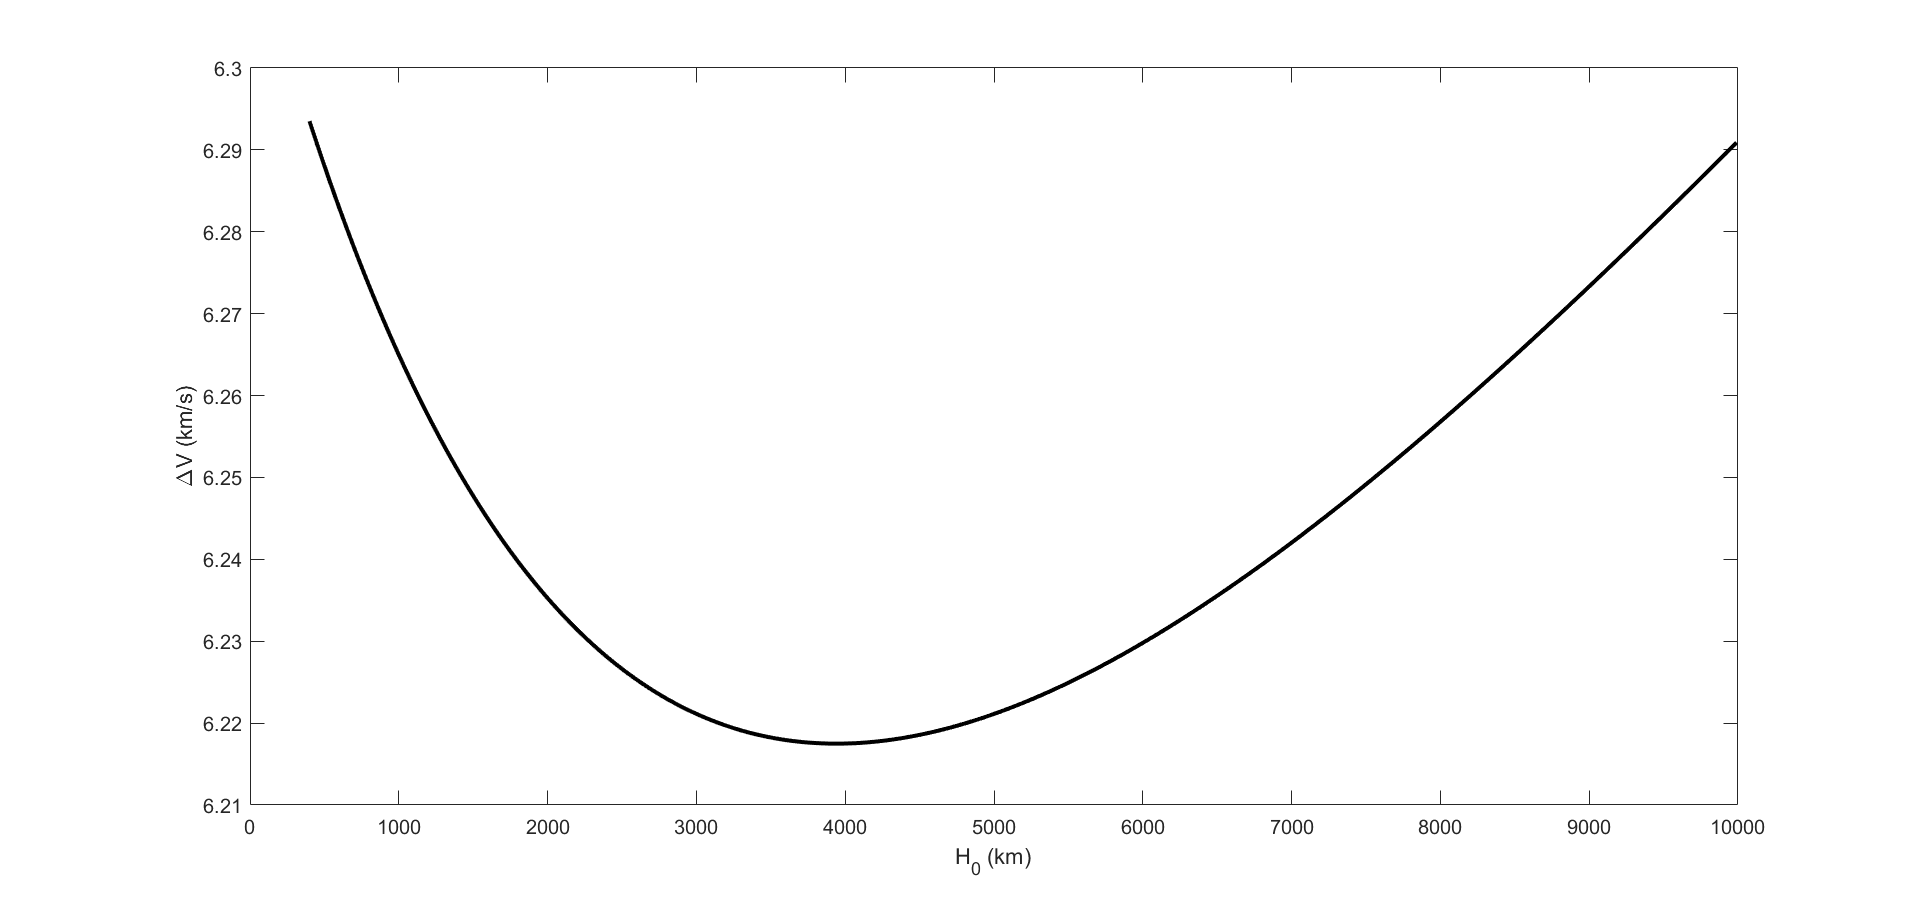
\includegraphics[width=\textwidth]{1b.png}
	\caption{$\Delta V$ vs $H_0$}
	\label{fig:1b}
\end{figure}

%%Figure 4
\subsubsection{Minimum $H_0$}
Thrust $\Delta V_{0J}$ is minimum when $H_0$ equals 3939 km (\fref{fig:1b}).From \fref{fig:1a} can be deduced that minimum $H_0$ of a parabolic scape path is at infinity.

\subsection{Direct transfer maneuver}

\begin{figure}[H]
	\centering
		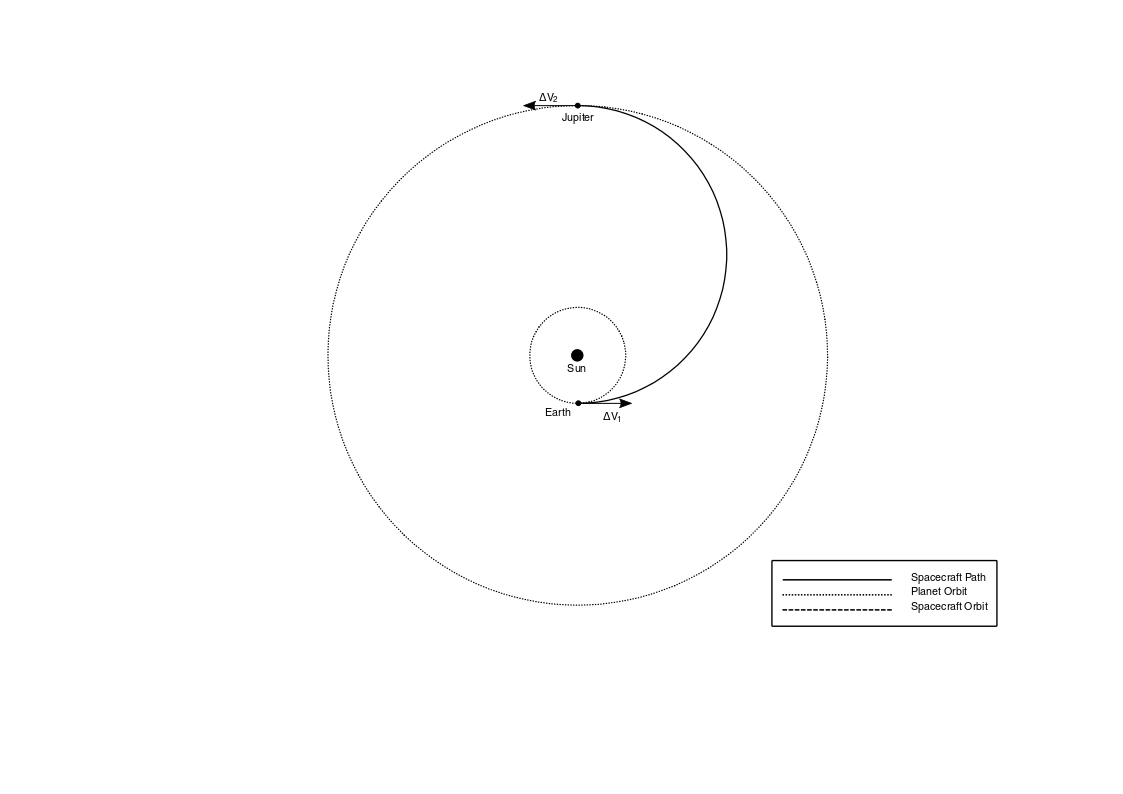
\includegraphics[width=\textwidth]{Hohman.png}
	\caption{Hohmann transfer maneuver $\Delta V$}
	\label{fig:Hohmann}
\end{figure}

In this part, the direct transfer maneuver from Earth to Jupiter will be developed. The main characteristic of this orbital maneuver is that the space vehicle traces a half elliptical orbit; in this case, with Jupiter orbital radius as apoapsis radius and Earth orbital radius as periapsis radius.To perform this Hohmann direct transfer maneuver two $\Delta V$ are needed. As seen in the figure above.  

The first $\Delta V$, ($\Delta V_1$) allows the vehicle to escape the orbit around the Earth, and places it in the transfer ellipse, with just one velocity impulse, as done in~\ref{sec:scape_maneuver}, using equation~\ref{eq:thrust22}. 

The second $\Delta V$, ($\Delta V_2$), applied in the ellipse apogee, will be the velocity that the vehicle has orbiting Jupiter minus the current velocity of the vehicle (velocity in the apogee of its elliptical orbit).

$$\Delta V_2 = \sqrt{\frac{\mu_{Sun}}{d_{SJ}}}-
\sqrt{2\mu_{Sun}\left(\frac{1}{d_{SJ}}-\frac{1}{2a}\right)}$$
  
The results are shown below:

\begin{itemize}

\item First impulse:

\begin{align*}
\Delta V_1&=\sqrt{\left(\sqrt{\left(\frac{2.654\times10^{11}}{1.5\times10^8}-\frac{1.327\times10^{11}}{4.643\times10^{8}}\right)}-\sqrt{\frac{1.327\times10^{11}}{1.5\times10^{8}}}\right)^2+\frac{7.972\times10^5}{6370+3939}}\\
&\quad-\sqrt{\frac{3.986\times10^5}{6370+3939}}
\end{align*}
$$\Delta V_1= 6.208 km/s $$

\item Second impulse:
$$\Delta V_2 = \sqrt{\frac{1.327\times10^{11}}{7.785\times10^8}}-
\sqrt{2\times1.327\times10^{11}\left(\frac{1}{{7.785\times10^{8}}}-\frac{1}{2\times 4.643\times10^{8}}\right)}$$

$$\Delta{V_2}= 5.633 km/s$$
\end{itemize}
The total velocity increment needed to perform the direct Hohmann maneuver can be obtained by adding both velocity increments.


\subsection{Insertion maneuver}

At this point, the vehicle has an orbital radius equal to Jupiter's orbital radius. The next step is to make the vehicle orbit Jupiter and put it into an orbit that has the same orbital radius than Jupiter's natural satellite Europa. 


The velocity of the vehicle at the apoapsis of its elliptical transfer orbit between the Earth and Jupiter:

 $$u_{a}=\sqrt{\mu_{Sun}\Big(\frac{2}{d_{SJ}}-\frac{1}{a}\Big)}=\sqrt{1.327\times10^{11}\Big(\frac{2}{7.785\times10^{8}}-\frac{1}{4.643\times10^{8}}\Big)} = 7.423 km/s$$
 
 
 By means of the law of conservation of energy, it is stated the energy of the vehicle  (with respect to Jupiter) has to remain the same before and after the gravitational influence. 
 
                $$\frac{(v_{\infty})^2}{2}=\frac{(v_{p})^2}{2}-\frac{\mu_{Jupiter}}{d_{Jupiter-Europa}}$$
                
                Where:
                $$v_{\infty}=u_{a-Jupiter}-u_{Jupiter}$$
                $$v_p=\Delta{V}+v_{vehicle}$$
                
 Thus: $$\frac{(u_{a-Jupiter}-u_{Jupiter})^2}{2}=\frac{(\Delta{V}+v_{vehicle})^2}{2}-\frac{\mu_{Jupiter}}{d_{Jupiter-Europa}}$$
 
 After operating:
               
               $$\Delta{V}=\sqrt{\Big(u_{a-Jupiter}-u_{Jupiter}\Big)^2+\frac{2\mu_{Jupiter}}{d_{Jupiter-Europa}}}-v_{vehicle}$$

\begin{equation}\label{eq:insertion}
\Delta{V}=\sqrt{\Big(u_{a-Jupiter}-\sqrt{\frac{\mu_{Sun}}{d_{SJ}}}\Big)^2+\frac{2\mu_{Jupiter}}{d_{Jupiter-Europa}}}-\sqrt{\frac{\mu_{Jupiter}}{d_{Jupiter-Europa}}}
\end{equation}

          
          {$$\Delta{V}=\sqrt{\Bigg(7.423 - \sqrt{\frac{1.327\times10^{11}}{7.785\times10^{8}}}\Bigg)^2+\frac{2\times1.267\times10^{8}}{6.71\times10^{5}}}-\sqrt{\frac{1.267\times10^{8}}{6.71\times10^{5}}}$$}
          
          $$\Delta{V} = 6.492 km/s$$
         
The needed time for the vehicle to arrive to Jupiter and orbit it can be estimated by means of Kepler's third law, which gives the period of the elliptical orbit. As only half of the elliptical orbit is traversed, the actual time will be half of the obtained period.

\begin{equation}
\frac{T^2}{a^3}=\frac{4\pi^2}{\mu}
\end{equation}

In this case, the time is:

$$t=\frac{1}{2}\sqrt{\frac{4\pi^2a^3}{\mu_{Sun}}}=\pi\sqrt{\frac{\left(d_{SE}+d_{SJ}\right)^3}{\mu_{Sun}}}$$
\begin{itemize}

\item The required time to execute the maneuver:
$$t=\pi\sqrt{\frac{\left(4.643\times10^{8}\right)^3}{1.327\times10^{11}}}= 2.74 years $$

This equation is just an approximation. Note that the needed time to perfom the insertion maneuver is neglected. It is only taken into account the time needed to perfom the Hohmann transfer shown in the previous section, eventhough the actual time would be obtained by adding both times. A more precise calculation is developed as a bonus part.

\end{itemize}


\subsection{Natural gravity assist} 
\begin{figure}[H]
	\centering
		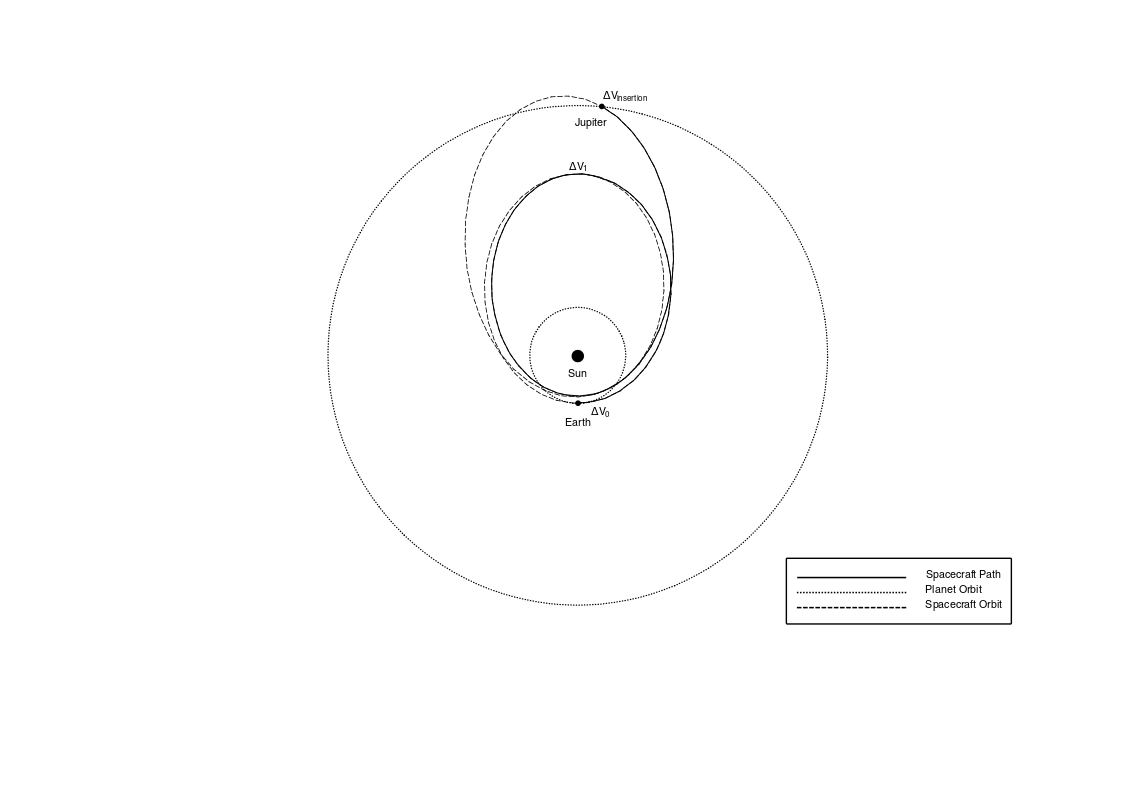
\includegraphics[width=\textwidth]{flyby.png}
	\caption{Earth to Jupiter for $H_\pi = 450km$}
	\label{fig:flybytrim}
\end{figure}

This maneuver consists of applying three speed increments. The first one is needed to escape the Earth, the second one to modify the trajectory and encounter the Earth to perform the gravitational assist maneuver and the last one, it will be a velocity increment to enter the orbit of Jupiter.

To begin, it is necessary to calculate satelite's scape speed with respect to the Sun ($u_{1p}$).
The spacecraft leaves the Earth with a hyperbolic orbit, that means that it will have an elliptical orbit around the sun. Let $v_s$ be the orbital speed of the satellite, $V_\infty$ is calculated by conservation of energy.

\begin{equation*}
V_\infty = \sqrt{(v_s + \Delta V_0)^2 - \frac{2 \mu_E}{R_E + H_0}}
\end{equation*}

Therefore, $u_{1p}$ is given by
\begin{equation*}
u_{1p} = V_\infty + u_E
\end{equation*}

Next, it is necessary to calculate the parameters of this ellipse, in this case the eccentricity and the apoapsis radius.

\begin{equation*}
e_1 = \frac{h_1^2}{\mu d_{SE}} - 1 
\end{equation*}

\begin{equation*}
d_{1a} = \frac{h_1^2}{\mu (1 - e)}
\end{equation*}

Knowing that $h_1=d_{SE}u_{1p}$.
Then, velocity at apoapsis $u_{1a}$ is calculated by means of the law of conservation of angular momentum.

At the apoapsis the brake thrust is applied, and the new speed will be $u_{2a} = u_{1a} + \Delta V_1$. Again, the parameters of the ellipse are needed.

\begin{equation*}
e_2 = 1 - \frac{h_2^2}{\mu d_{1a}}  
\end{equation*}

\begin{equation*}
d_{2p} = \frac{h_2^2}{\mu(1 + e)}
\end{equation*}

u1This new orbit intersects the Earth's orbit at an angle $\theta_i$, which is the true anomaly of the orbit at the intersection point, where the spacecraft's orbital radius equals to the Earth orbital radius.

\begin{equation}
\theta_i = \arccos\left[\frac{a_2(1-e_2^2)- d_{SE}}{e_2d_{SE}}\right]
\end{equation}

The last equation has two different solutions (two different angles), but there will be just one correct answer, the one that gives a tangent velocity at that point. 

\begin{equation}
\vec{u_s}^- = \sqrt{\frac{\mu_S}{a2(1 - e_2^2)}}
\left(
\begin{array}{c}
-\sin\theta_i\\
e_2 + \cos\theta_i
\end{array}
\right)
\end{equation}

Earth's speed vector is
\begin{equation*}
\vec{u_E} = \sqrt{\frac{\mu}{d_{SE}}}
\left(
\begin{array}{c}
-\sin\theta_i\\
\cos\theta_i
\end{array}
\right)
\end{equation*}

Therefore, the speed of the spacecraft with respect to the Earth before the assist is:
\begin{equation*}
\vec{v}^-_\infty = \vec{u_s}^- - \vec{u_E}
\end{equation*}

And the speed after the assist with respect to the Sun will be
\begin{equation}\label{eq:uplus}
\vec{u_s}^+ = \vec{v}^+_\infty + \vec{u_E}
\end{equation}

As the spacecraft describes a hyperbolic path around the Earth, if the law of conservation of the energy is applied, the result is $v_\infty^- = v_\infty^+$. Speed modulus with respect to the Earth is the same before and after the maneuver, but the direction of the vector changes.

\begin{equation}
\vec{v}^+_\infty = R(\delta)\vec{v}^-_\infty
\end{equation}

The rotation matrix is

\begin{equation*}
R(\delta) = \left(
\begin{array}{cc}
\cos\delta & -\sin\delta \\
\sin\delta & \cos\delta
\end{array}
\right)
\end{equation*}

where $\delta$ is the angle between the speed vector at the entry and exit.

\begin{equation*}
\delta = 2\left(\pi - \arcsin\left(\frac{1}{e_{hyp}}\right)\right)
\end{equation*}

and 
\begin{equation*}
e_{hyp} = 1 + \frac{r_\pi v_\infty^2}{\mu_E}
\end{equation*}

It can be seen that the speed after the fly-by maneuver (given by \eqref{eq:uplus})  is a function of $H_\pi$, as $r_\pi = R_E + H_\pi$.

Now, the parameters of the approach orbit are required. Apoapsis radius can be calculated by
\begin{equation}\label{eq:d3a}
d_3a = \frac{h_3^2}{\mu(1-e)}
\end{equation}

where the eccentricity is given by

\begin{equation}\label{eq:e_ellipse_urmu}
\vec{e} = \frac{\left(\vnorm{u}^2 - \frac{\mu}{\vnorm{r}}\right) \vec{r} - \left(\vec{r}\cdot\vec{u}\right) \vec{u}}{\mu}
\end{equation}

By operating \eqref{eq:e_ellipse_urmu} and substituting in \eqref{eq:d3a} the value is calculated.

Finally, it is necessary to calculate the total thrust.

\begin{equation*}
\Delta V_T = \Delta V_0 + \Delta V_1 + \Delta V_{insertion}
\end{equation*}

Where $\Delta V_{insertion}$ is calculated with \eqref{eq:insertion}. 

To minimize this non-linear multi-variable function it would be necessary to use numerical methods. For example, a genetic algorithm could be implemented.

\begin{figure}[H]
	\centering
		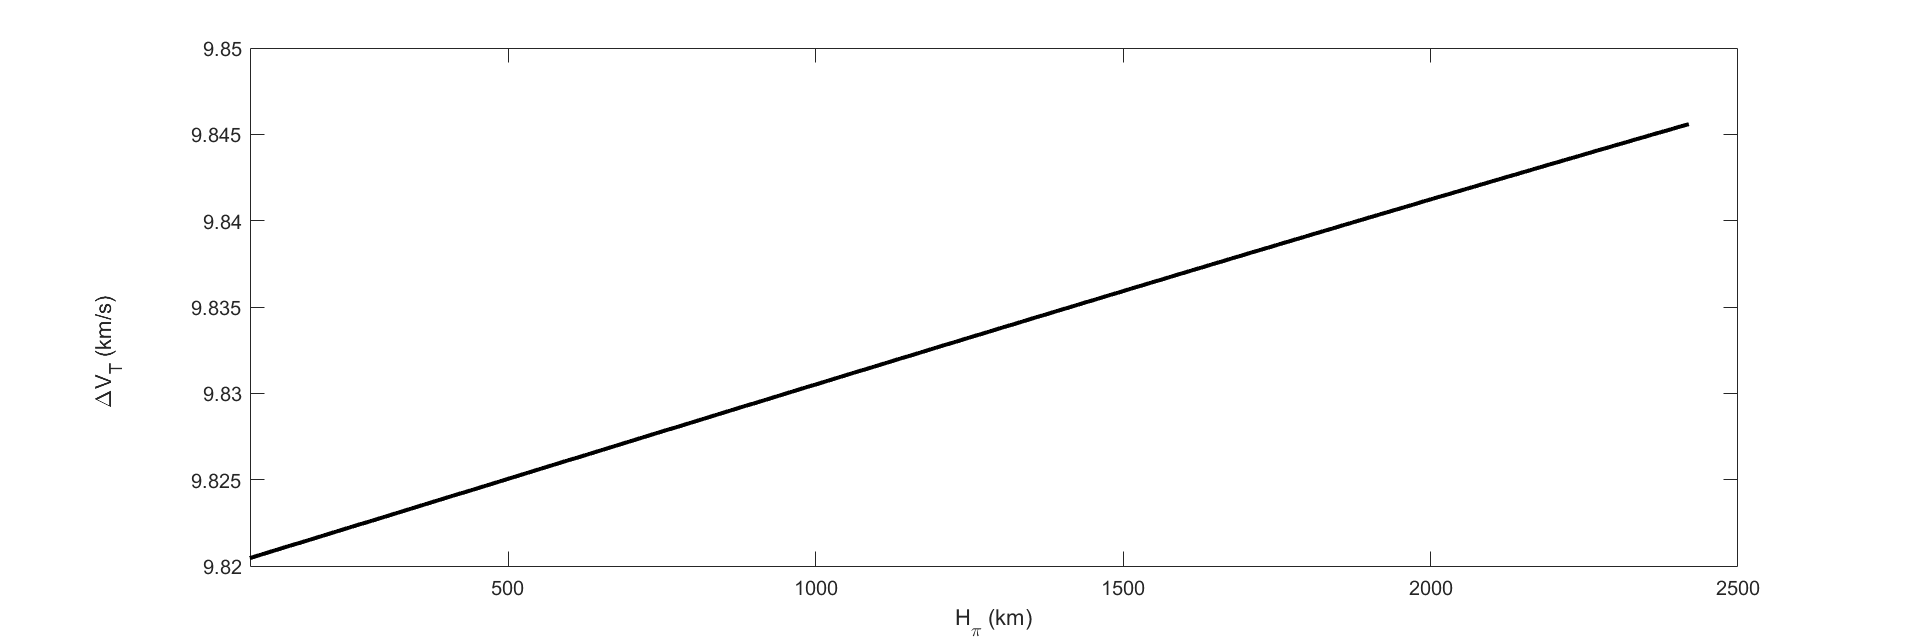
\includegraphics[width=\textwidth]{untitled.png}
	\caption{$\Delta V_T$ vs $H_\pi$}
	\label{fig:2b}
\end{figure}

% REGULA FALSI 


\subsection{Jupiter travel's Time}
Kepler's equation, wich relates various geometric properties of the orbit of a body subject to a central force, is defined by:
\begin{equation}\label{eq:Kepler}
M=E-esinE
\end{equation}
where $E$ is the eccentric anomaly,
$M$ is the mean anomaly and $e$ is the eccentricity of the orbit:
\begin{equation*}
e=\frac{r_pv_p^2}{\mu}-1
\end{equation*}
\begin{equation*}
E=\arccos\left(\frac{e+cos\theta}{1+ecos\theta}\right)
\end{equation*}
\\
Knowing that $M$ depends of the travel time, it can be isolated:
\begin{equation}\label{eq:m_anomaly}
M=\sqrt{\frac{\mu}{a^3}}(t-\tau)
\end{equation}
where 
\begin{equation*}
a=\frac{r_p^2v_p^2}{\mu (1-e)}
\end{equation*}
\\
and $\tau$ is the time at which the body is at the periapsis. From~\eqref{eq:Kepler} and~\eqref{eq:m_anomaly}:

\begin{equation*}\label{eq:130}
E-esinE=\sqrt[]{\frac{\mu}{a^3}}(t-\tau)
\end{equation*}
\\
Setting $\tau=0$ 
\begin{equation}\label{eq:temps}
t=(E-esinE)\sqrt{\frac{a^3}{\mu}}
\end{equation}

To calculate the travel time from the last section the expresion \eqref{eq:temps} will be used. 
It can be divided in three parts: travel time to reach the apoapsis of the first orbit ($t_1$), time to travel from the apoapsis back to Earth ($t_2$), and time from Earth to Jupiter after the gravity assist ($t_3$). Gravity assist and insertion maneuvers' time will be considered negligible.
\begin{equation*}
t_{T}=t_{1}+t_{2}+t_{3}
\end{equation*}
$t_{1}$ is easily calculated directly aplying the formula for $\theta=\pi$:
\begin{equation*}
t_1=(E_1-e_1sinE_1)\sqrt{\frac{a_1^3}{\mu_S}} % CALCULAR
\end{equation*}

$t_{2}$ can be calculated by adding the time needed to reach the Earth from the periapsis and the time needed to reach the periapsis from the apoapsis. Due to the symetry of the orbit, the latter one is equal to the time to needed to reach the apoapsis from the periapsis.
\begin{equation*}
t_2=(E_{2;\theta=\pi}-e_2sinE_{2;\theta=\pi}+E_{2;\theta=\theta_{int}}-e_2sinE_{2;\theta=\theta_{int}})\sqrt{\frac{a_2^3}{\mu_S}} % CALCULAR --> ANGLEEE
\end{equation*}

Lastly, $t_3$ is calculated by substracting the time from the periapsis to the intersection point from the time from the periapsis to Jupiter in Jupiter's approach orbit. 
\begin{equation*}
t_3=(E_{3;\theta=\theta_J}-e_3sinE_{3;\theta_J}-(E_{3;\theta=\theta_{int}}-e_3sinE_{3;\theta=\theta_{int}}))\sqrt{\frac{a_3^3}{\mu_S}} % CALCULAR --> ANGLEEE (Respecte a la nova òrbita)
\end{equation*}

That way it can be seen that $\tau=0$ and there is no need to calculate it. \\

$\theta_J$ is the angle of intersection with Jupiter. This can be done with:

\begin{equation*}
\cos{\theta} = \frac{\vec{e}\cdot\vec{r}}{\vnorm{e} \vnorm{r}}
\end{equation*}
% ESQUEMA ÒRBITES 1, 2, 3

Total travel time to reach Jupiter:
\begin{equation*}
t_T = 1.03 + 1.08 + 2.72 = 4.83 years
\end{equation*}

\nocite{franchini2008introduccion}
\nocite{curtis2013orbital}